\documentclass{article}
\usepackage{tikz}
\usetikzlibrary{graphs, graphs.standard, quotes}

\begin{document}

\begin{figure}[h]
    \centering
    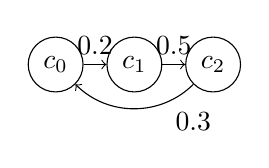
\begin{tikzpicture}
        \graph [simple] {
            c0 [as=$c_0$, shape=circle, draw] -> ["0.2"] c1 [as=$c_1$, shape=circle, draw] -> ["0.5"] c2 [as=$c_2$, shape=circle, draw];
            c2 -> [bend left=45, "$0.3$", near start] c0;
        };
    \end{tikzpicture}
    \caption{An example of a graph that represents a stochastic compartmental model with 3 compartments. The label of the $(c_2, c_0)$ edge is a vector with $0.3$ indexed by $c_1$ and all other values are zero (thus omitted to avoid clutter).}
    \label{fig:stochastic_compartmental_model}
\end{figure}

\end{document}